\chapter{Introduzione alla misura dei parametri}
Nel caso dei sistemi biometrici non è banale rispondere alla domanda: \textit{\textbf{
    "qual è il tasso di errore di verifica/identificazione?"
}}

Per descrivere le performance del sistema è necessario disporre di \textbf{un insieme di dati} e \textbf{curve di funzionamento};
per questo motivo diventa difficile comparare due sistemi in quanto non basta confrontare 2 numeri.

\subsubsection{Genuini ed impostori}

Si impiegano i termini:
\begin{itemize}
    \item \textbf{genuino} per indicare un individuo che accede al sistema e ha titolo per farlo
    \item \textbf{impostore} per chi prova ad accedere senza averne titolo
\end{itemize}

La formulazione del problema risulterà diversa a seconda che il sistema funzioni in \textbf{verification} o \textbf{identification}.

\newpage

\section{Verifica e Identificazione}

\subsection{Verifica}

\textit{"tu sei chi dici di essere?"}
\\
Il problema in questo caso si riconduce ad un caso di classificazione binaria.

\subsubsection{Problema della verifica}

Dato in ingresso un insieme di caratteristiche $X_Q$ e la dichiarata identità $I$,
occorre determinare se $(I, X_Q)$ appartiene a $w_1$ o $w_2$, dove:
\begin{itemize}
    \item $w_1$ indica che la richiesta è vera (utente genuino)
    \item $w_2$ indica che la richiesta è falsa (un impostore)
\end{itemize}

Tipicamente, le caratteristiche $X_Q$ vengono controllate con le caratteristiche $X_I$ (il template associato alla identità $I$).

\subsubsection{Regola di decisione per la verifica}

Si tratta di una comparazione con soglia:
\begin{figure}[ht]
    \centering
    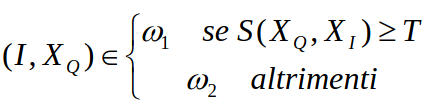
\includegraphics[width=0.5\linewidth]{chapters/images-chap2/regola-verifica.png}
\end{figure}

Dove:
\begin{itemize}
    \item $S$ è la funzione che misura la similitudine tra $X_Q$ e $X_I$
    \item $T$ è la soglia prefissata
    \item $S(X_Q, X_I)$  prende il nome di \textbf{match score}
\end{itemize}

\subsection{Identificazione}
\textit{"il sistema controlla se i tuoi dati biometrici corrispondono
 ad un insieme di identità registrate"}

\subsubsection{Problema di identificazione}
Dato in ingresso un insieme di caratteristiche $X_Q$, determinare l'identità 
$I_k$, con $k \in \{1,2,3,...,M,M+1\}$ dove $I_1, I_2,...,I_M$ sono 
le M identità memorizzate nel sistema e $I_M+1$ rappresenta il \textbf{caso di reiezione}.

Nel caso di reiezione nessuna delle M identità registrate è sufficientemente simile al dato in ingresso.

\newpage

\subsubsection{Regola di decisione per l'identificazione}
Si tratta di M comparazioni con soglia con la seguente regola di decisione:
\begin{figure}[ht]
    \centering
    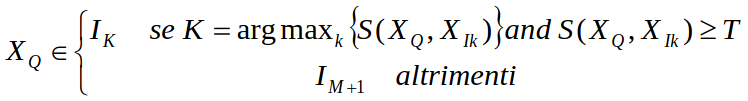
\includegraphics[width=1\linewidth]{chapters/images-chap2/regola-identificazione.png}
\end{figure}

Dove:
\begin{itemize}
    \item $X_Ik$ è il template corrispondente alla identità $I_k$
    \item $T$ è la soglia prefissata
    \item $S(X_Q, X_I)$ prende il nome di \textbf{match score}
\end{itemize}

In alcuni casi ci si riferisce ad una \textbf{misura della distanza} fra
$X_Q$ e $X_I$; una \textbf{grande distanza} fra i vettori di features porta ad un \textbf{basso match score}.

\section{Distanza tra template}

N template, provenienti dalla stessa persona ma acquisiti in tempi diversi,
NON sono \textbf{mai uguali}.

Esiste sempre una distanza nello spazio delle features che separa i template anche della 
stessa persona (rumore, posa del soggetto, illuminazione, condizione ambientiali, \dots)

Questa comporta che \textbf{la soglia $T$ non può esser arbitrariamente abbassata}, altrimenti 
nessuno sarebbe identificato.

Se si riscontrasse una \textbf{distanza nulla} fra $X_Q$ e $X_I$ (quindi $S(X_Q, X_I) = max$), probabilmente 
saremmo di fronte ad un \textbf{replay attack}: una copia illecita di un template memorizzato che viene 
riproposto per frodare un sistema.

\subsubsection{Genuini ed impostori}

Si parla di \textbf{\textcolor{green}{genuine score}} quando si confrontano le distanze tra i template
dello stesso individuo.

Si  parla di \textbf{\textcolor{red}{impostor score}} quando si confrontano le distanze tra i template 
di indivdui diversi.

\newpage

\subsection{Distribuzioni dei match score}

\begin{figure}[ht]
    \centering
    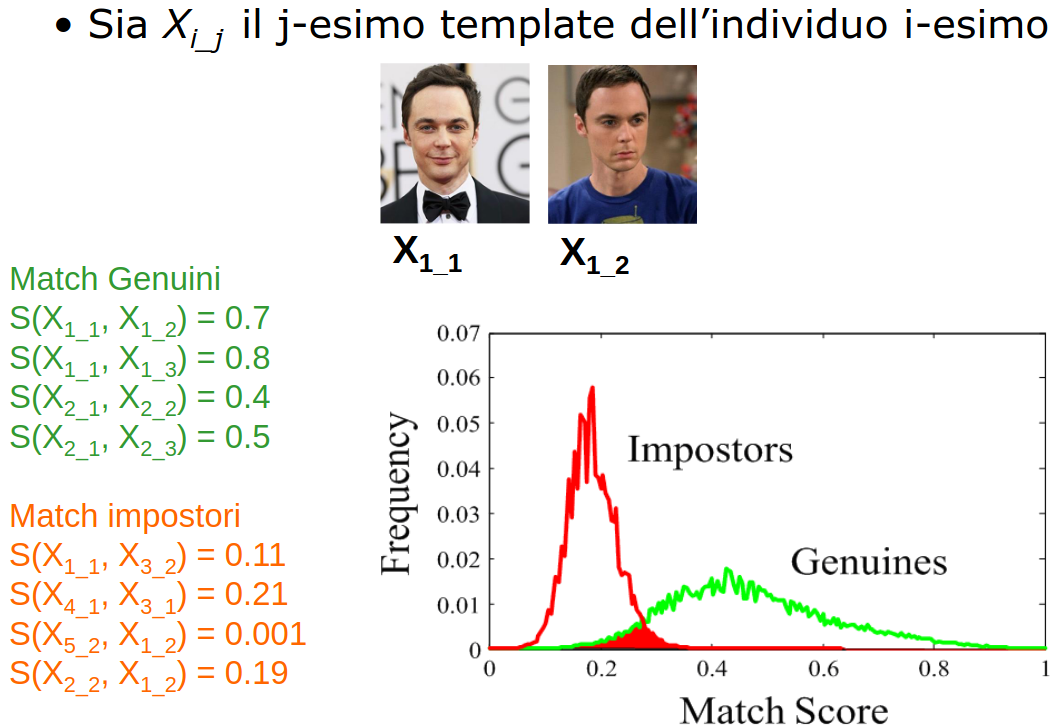
\includegraphics[width=1\linewidth]{chapters/images-chap2/distr-matchscore.png}
\end{figure}

\section{False Match e False Non-Match}

\begin{itemize}
    \item \textbf{False Match:} \textit{il ladro entra in casa perché il sistema lo 
    ha scambiato per noi;} \textbf{$impostorScore > T$}
    \item \textbf{False Non-Match:} \textit{non entrate in casa perché il sistema ritiene che il template non assomigli
    abbastanza a quello/i registrati;} \textbf{$genuineScore < T$}
\end{itemize}

\subsection{FM Rate, FNM Rate}

Supponiamo di poter variare la soglia e di fissarla a un valore $T$ in mezzo fra il picco
degli impostori e quello dei genuini. Notiamo che:
\begin{itemize}
    \item un certo numero di persone appartenenti al gruppo dei \textbf{\textcolor{green}{genuini}} 
    sono \textbf{sotto la soglia T}; non saranno autorizzati e daranno errore di
    False Non-Match (FNM).

    \textit{FNMR(T) = FNM(T) / numGenuini}
    \item una parte degli \textbf{\textcolor{red}{impostori}} hanno valori di match
    \textbf{sopra la soglia T}; saranno autorizzati e daranno errori di False Match (FM).

    \textit{FMR(T) = FM(T) / numImpostori}
\end{itemize}

\begin{figure}[ht]
    \centering
    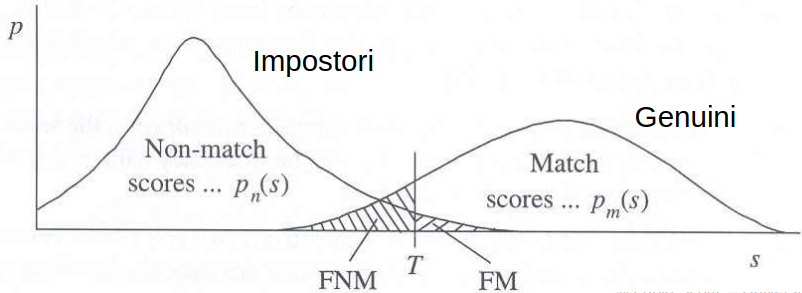
\includegraphics[width=1\linewidth]{chapters/images-chap4/rate.png}
    \caption{FNM e FM}
    \label{fig:rate}
\end{figure}

Il funzionamento di un sistema biometrico dal punto di vista degli errori commessi 
è descritto dai tassi \textit{FMR(T)} e \textit{FNMR(T)} per tutti i valori della soglia.

\section{Decision Error Tradeoff (DET) e Receiver Operating Characteristic (ROC)}

\subsubsection{DET: Regioni di funzionamento}
Regolando la soglia T possiamo regolare il livello di sicurezza.

\begin{figure}[ht]
    \centering
    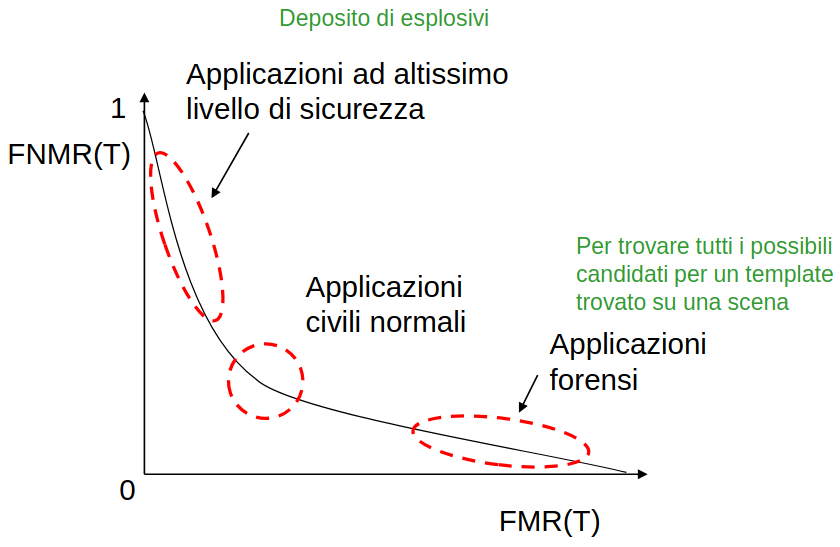
\includegraphics[width=1\linewidth]{chapters/images-chap4/det.png}
\end{figure}

\subsubsection{DET: Equal Error Rate}

L'EER è il tasso di errore corrispondente all'unico punto nel
quale si ha FNMR = FMR.

Si tratta dell'unico numero singolo che può riassumere il funzionamento del sistema.

\subsubsection{ROC = 1 - DET}

\textbf{La curva DET e ROC mostrano le stesse informazioni}.
La DET mette l'attenzione sul FNM (genuini che non entrano), mentre la ROC 
mette l'evidenza su 1 - FNM (quanti genuini riescono ad entrare).

\begin{figure}[ht]
    \centering
    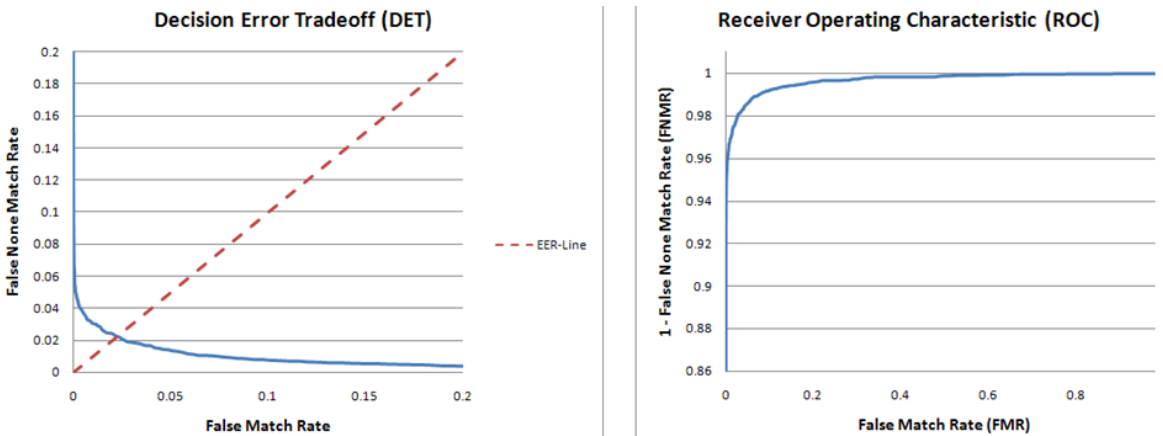
\includegraphics[width=1\linewidth]{chapters/images-chap4/det-roc.png}
    \caption{Curve DET e ROC}
\end{figure}

\section{Metodi statistici per la stima dei parametri in
un sistema biometrico}

\subsection{Che modello usiamo?}

Chiariamo il concetto di \textbf{Prova/Esperimento di Bernoulli:}
\begin{enumerate}
    \item ad ogni singola prova si hanno solo due esiti possibili
    \begin{itemize}
        \item successo (1)
        \item insuccesso (0)
    \end{itemize}
    \item La probabilità \textbf{\textit{p}} dell'evento 'successo' è costante
    \item i risultati delle prove sono \textbf{indipendenti}
\end{enumerate}

Date due impronte il SB in autenticazione mostra un tasso di errori stimabile e fissato \textit{\textbf{p}}.

L'evento che il SB sbagli una autenticazione è un \textbf{esperimento/prova di Bernoulli}.

Un SB usato in identificazione (1:N) si può modellizzare come un N prove di Bernoulli, 
ovvero un \textbf{processo di Bernoulli}.

\subsection{Regola dei 3}

\textit{"qual è il tasso di errore più basso p che può essere stimato con un esperimento
di comparazione di N campioni indipendenti?"}

Se abbiamo un sistema che commette 0 errori su N prove non dobbiamo pensare di
avere un sistema con $p=0$, ma con il 95\% di confidenza abbiamo un sistema
che ha $p \approx 3/N$.

\subsubsection{Esempio}

Se faccio 300 prove e ho 0 errori, allora posso dire con confidenza del 95\% che
il sistema ha un tasso di errore stimato del $p \approx 3/N = 3/100 = 1\%$

\subsection{Regola dei 30}

La regola dei 30 è utilizzata per determinare la larghezza del campione biometrico in questo modo:

per essere sicuro con intervallo di confidenza del 90\% che il tasso di errore \textbf{vero}
sia tra il $\pm 30 \%$ del tasso di errore \textbf{osservato}, ci devono essere almeno 30 errori.

\subsubsection{Esempio}
Se abbiamo 30 FNM in 3000 comparazioni, possiamo dire (con intervallo di 
confidenza del 90\%) che l'errore vero sia tra $0,7\%$ e $1,3\%$.